Si attribuisce a Vapnik l'applicazione fruttuosa
del kernel all'apprendimento automatico (1992).

\subsection{Il Kernel}
Prende il nome da qualche teoria matematica avanzata.
Per capirsi
\subparagraph{Il prodotto scalare \`e un kernel} Presi due vettori, due elementi di uno spazio
in cui sia definito un prodotto scalare,
il kernel sar\`a un'estensione del prodotto scalare consueto
\subparagraph{Il kernel \`e un prodotto scalare} L'idea è
di portarsi in un comodo spazio dotato di prodotto scalare
per poi applicare il kernel


Formalmente:
\begin {equation}
  \label {eq:kernel}
  k = \langle \mathbf{\Phi}(x_1), \mathbf{\Phi}(x_2) \rangle
\end{equation}
dove $\mathbf{\Phi}(x)$ \`e una mappa -se si vuole- non lineare
che porta i generici elementi $x$
in uno spazio dotato di prodotto scalare.

NB$_{1}$: Gli elementi originali possono quindi non essere neanche vettori.\par
NB$_{2}$: In generale \`e pi\`u semplice scrivere la funzione kernel piuttosto che la mappa.\par
Oss: Praticamente si stanno estraendo le caratteristiche.\par

\subsubsection{Il kernel e l'apprendimento automatico}
Rimanendo nell'ambito della classificazione binaria
la funzione discriminante \`e
\begin{equation}
	\label{eq:discriminante}
	y_n = sgn \left(\langle w, \mathbf{\Phi}(x_n) \rangle + b \right)
\end{equation}
ma si definiscono i pesi come
\begin{equation}
  \label{eq:pesikernel}
  w = \sum_i y_i \alpha_i \mathbf{\Phi}(x_i)
\end{equation}
con $\alpha_i$ che \textbf{come si chiama?}
Sostituendo la \ref{eq:pesikernel} nella \ref{eq:discriminante}
si ottiene
\begin{align}
  y_n &= sgn \left(\sum_i y_i \alpha_i \langle \mathbf{\mathbf{\phi}}_i,\mathbf{\mathbf{\phi}}_n \rangle + b \right) \\
  &= sgn \left(\sum_i y_i \alpha_i k(x_i,x_n) + b \right)
  \label{eq:uscitakernel}
\end{align}

\subsubsection {Il kernel perceptron}
(Tratto da un articolo dell'Universit\`a di Trento).
L'algoritmo di apprendimento \`e molto simile
a quello del percettrone classico.
La differenza sta nel calcolo della funzione (vedi eq. precedente)
e nell'aggiornamento dei pesi:
gli $\alpha_i$ sono incrementati ogni volta che
il neurone sbaglia la previsione su un $x_i$.


\subsubsection {\acf{spra}}
Schoelkopf e Smola propongono un semplice algoritmo di classificazione
introduttivo alle macchine a vettori di supporto (\ac{svm}).

Non si fa altro che prendere i punti medi delle due classi ($c_1$ e $c_2$),
prendere il vettore differenza trai due $w=c_1-c_2$
il loro punto medio ($c=(c1+c2)/2$).

Ora ogni altro punto di classe ignota
pu\`o essere etichettato con
\(y =sgn \left( \langle \boldsymbol{x-c}, \boldsymbol{w} \rangle \right)\).



\subsection {\acf{svm}}
Sono algoritmi che usano l'espediente del kernel
per mappare le sequenze in degli spazi comodi
(tipicamente con molte dimensioni in pi\`u)
dove trovare il piano di separazione che massimizza il margine (\textsc{Figura~\ref{fig:clus_svm}}).
Nello spazio di partenza la separazione pu\`o assumere le forme pi\`u diverse
(dipende dalla mappa non lineare).

Il problema \`e posto nei termini di minimizzazione della lagrangiana
\begin{equation}
    L_P = lagrangiana
  \label{eq:lagrangiana}
\end{equation}
o massimizzazione della sua duale
\begin{align}
  \label{eq:lagr_duale}
  L_D &= \sum_i \alpha_i - \frac{1}{2} \sum_i \sum_j \alpha_i \,\alpha_j \,y_i \,y_j \,k(\boldsymbol{x_i}, \boldsymbol{x_j}) \\
  \langle \boldsymbol{\alpha}, \boldsymbol{y} \rangle &= 0 \\
  \alpha_i &\geq 0
\end{align}

\begin{figure}
\centering
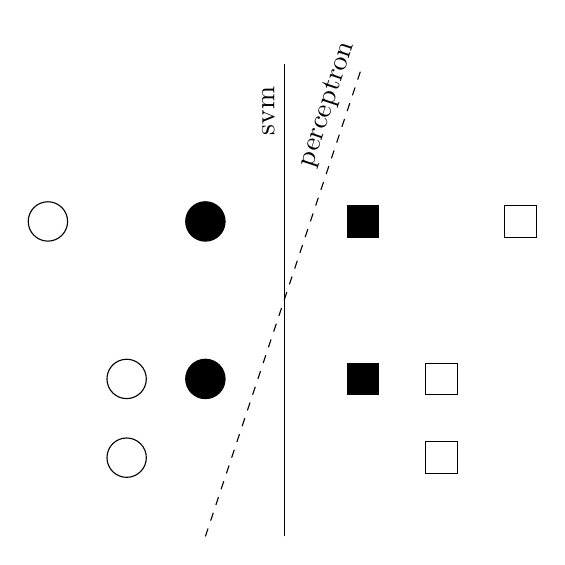
\begin{tikzpicture}

% \draw (-8, -5) grid (5, 5);

\draw [fill] (-1,1) circle (.25);
\draw [fill] (-1,-1) circle (.25);
\draw (-2,-1) circle (.25);
\draw (-2,-2) circle (.25);
\draw (-3,1) circle (.25);

\draw [fill] (1,1) ++(-.2,-.2) rectangle ++(.4,.4);
\draw [fill] (1,-1) ++(-.2,-.2) rectangle ++(.4,.4);
\draw (2,-1) ++(-.2,-.2) rectangle ++(.4,.4);
\draw (2,-2) ++(-.2,-.2) rectangle ++(.4,.4);
\draw (3,1) ++(-.2,-.2) rectangle ++(.4,.4);

\draw [dashed] (-1,-3) -- (1,3)
 node[pos=.9,sloped,above]{perceptron};
\draw (0,-3) -- (0,3)
 node[pos=.9,sloped,above]{\acs{svm}};

% \draw (-5,-2) circle (.125);
% \draw (-5,-1) circle (.125);
% \draw (-6,-1) circle (.125);
% \draw (-6,-2) circle (.125);
% \draw (-7,-2) circle (.125);

% \draw (-6.5,-1.3) ++(-.1,-.1) rectangle ++(.2,.2);
% \draw (-6,0) ++(-.1,-.1) rectangle ++(.2,.2);
% \draw (-6.7,-3) ++(-.1,-.1) rectangle ++(.2,.2);
% \draw (-5.5,-3.4) ++(-.1,-.1) rectangle ++(.2,.2);
% \draw (-4.7,-2.1) ++(-.1,-.1) rectangle ++(.2,.2);

% \draw [->, ultra thick] (-4.5, -2.5) -- (-2, 0)
%   node [pos=.5, sloped, above] {mappa $\Phi$};

\end{tikzpicture}
\caption{L'\acs{svm} trova il piano di separazione che massimizza il margine}
\label{fig:clus_svm}
\end{figure}

\subsubsection{Ottimizzazione con MatLab}
Per eseguire lquesta operazione si utilizza la funzione
\(fmincon\) di ottimizzazione vincolata.

\par
Questa strumento prende in ingresso
la funzione obiettivo e la funzione supporto,
vale a dire la funzione da minimizzare e i vincoli non lineari da rispettare;
il punto di partenza;
gli eventuali vincoli lineari di uguaglianza e disuguaglianza.


